\documentclass{article}
\usepackage[preprint]{neurips_2025}
\usepackage[utf8]{inputenc}
\usepackage[T1]{fontenc}
\usepackage{hyperref}
\usepackage{url}
\usepackage{booktabs}
\usepackage{amsfonts,amsmath}
\usepackage{nicefrac}
\usepackage{microtype}
\usepackage{xcolor}
\usepackage{graphicx}
\usepackage{subcaption}
\usepackage{tikz}
\usetikzlibrary{positioning,arrows.meta,fit,calc,shapes.geometric}

\newcommand{\SE}{\mathrm{SE}}
\setlength{\textfloatsep}{12pt plus 2pt minus 4pt}
\setlength{\abovecaptionskip}{6pt}
\makeatletter\renewcommand{\@noticestring}{}\makeatother

\title{Does the Model Know What to Forget? Measuring Uncertainty in Self-Managed Context}

\author{%
  Eben Lim\\
  Nanyang AI Safety, Nanyang Technological University\\
  \texttt{ebenlim08@gmail.com}\\[8pt]
  \textbf{With}\\
  Apart Research
}

\begin{document}
\maketitle
\vspace{-0.2in}

\begin{abstract}
  Language models are beginning to manage their own memory.
  In a Context Language Model (CLM), the model decides at every turn which parts of its transcript to keep, cut, or move to disk, and a wrong decision can silently discard information the task later needs.
  We ask whether the model is uncertain when it makes the decisions that later cost it the task, and whether it carries that uncertainty internally.
  We first reproduce the problem on ContextBench.
  As the input grows from half to 24 times the context window, Qwen3.5-9B's reward falls from 0.95 to 0.12.
  Most failed trials fill their context before finishing, and some finish with answers built on batches that were dropped rather than saved.
  We then replay 42 logged trials exactly, ask the model to make each of about 1{,}400 context decisions ten times, run every resulting command, and group the outcomes by what they did to the context.
  The spread of these outcomes, their semantic entropy, measures the model's total uncertainty about each decision.
  Trials with more uncertain decisions fail more often at the same input length (partial $\rho=-0.59$), and the pattern holds for an RL-trained version ($\rho=-0.48$) and when broken commands are excluded.
  The uncertainty is also visible before the model acts: a linear probe on its activations predicts it with AUROC 0.74--0.82, against 0.49--0.58 for a context-length baseline.
  A correlation between the model's total uncertainty and its ContextBench performance therefore hints at a potentially new method
  for a more explicit control of model's way in context handling.
\end{abstract}

%=====================================================================
\section{Introduction}
%=====================================================================

Long-horizon agents produce more text than any fixed context window can hold, so some component must decide what remains in context, what is compressed, and what is discarded.
Until recently that component was the harness: a fixed rule truncated or summarised the transcript.
Context Language Models (CLMs) \citep{shao2026clm} move the decision into the model.
The context is exposed as a file that the model edits with ordinary commands, so the model itself chooses, turn by turn, which earlier messages to keep, shorten, offload to disk, or delete.

Moving context management into the model changes what a failure means.
When a CLM agent fails on a long task, the failure is the outcome of a sequence of judgements made by the model, and each judgement can be wrong in ways that cannot be undone: a value deleted rather than offloaded is lost, and a file overwritten destroys earlier work.
Whether such an agent can be trusted therefore depends in part on whether the model represents its own uncertainty about these decisions.
A model that is uncertain and knows it offers a signal that can be measured and acted upon; a model that is uncertain without any internal trace of that uncertainty fails silently.

Prior work establishes that performance degrades as context grows \citep{du2025context}, and our reproduction confirms that CLM reward falls as the input outgrows the context budget.
Pressure explains the average decline but not which trials fail: at the same pressure level, some trials succeed while others fill their context or lose information they later need.
We test whether the model's uncertainty about its own context decisions accounts for this variation.
Our measure is semantic entropy \citep{kuhn2023semantic,farquhar2024detecting}, adapted from text to actions: two sampled replies are equivalent when they have the same effect on the context, regardless of how the commands are written.

We address three questions, one per experiment.
\textbf{Elicitation} (Experiment~1, Section~\ref{sec:exp1}): does a reimplemented CLM agent fail under context pressure, and is the failure one of context management?
\textbf{Correlation} (Experiment~2, Section~\ref{sec:exp2}): does the semantic entropy of context decisions predict task failure beyond pressure level?
\textbf{Decodability} (Experiment~3, Section~\ref{sec:exp3}): is this uncertainty linearly readable from the model's activations before it generates a reply?

Our contributions are fourfold.
(i) We reproduce a pressure-dependent failure of CLM agents on ContextBench across three Qwen3.5 models and trace it to context management.
(ii) We measure decision uncertainty through execution: byte-exact replay of logged trials, resampling at each decision point, execution of every sample, and clustering by effect on the context.
(iii) We show that this uncertainty predicts failure at fixed pressure in a base model and its RL-trained variant, also when command failures are removed.
(iv) We show that a linear probe reads it from the residual stream before generation, well above a context-length baseline.
All experiments were conducted during the research sprint; code and data are available at \url{https://github.com/ebenl08/clm-epistemics/}.

%=====================================================================
\section{Related work}
%=====================================================================

\textbf{Context management by the model.} \citet{shao2026clm} introduce CLMs, in which the context is a file the model may edit without restriction, and release ContextBench, a benchmark that streams more data than fits in context and measures what an agent keeps, updates, and offloads.
They also train an RL checkpoint of Qwen3.5-9B for context management, which we use.

\textbf{Long-context degradation.} \citet{du2025context} show that performance falls with input length even when retrieval is perfect, so any signal that correlates with failure must be tested against context length.
We include context fill as a control throughout.

\textbf{Semantic entropy.} \citet{kuhn2023semantic} propose semantic entropy, which clusters sampled generations by meaning and computes entropy over clusters rather than tokens; \citet{farquhar2024detecting} use a discrete variant to detect hallucinations.
We keep the discrete estimator and replace meaning-equivalence of text with equivalence of effects on the context.

\textbf{Probing and steering.} \citet{kossen2024sep} train linear probes that predict semantic entropy from hidden states, and find that the hidden state before generation already carries the signal.
We follow their probe design and token positions.
\citet{marks2023geometry} find that difference-of-means directions tend to be more causally implicated than probe weights, and \citet{arditi2024refusal} ablate a single residual-stream direction by orthogonalising the weights.
We use both in the preliminary intervention of Appendix~\ref{app:h3}.

%=====================================================================
\section{Setting}
\label{sec:setting}
%=====================================================================

\begin{figure}[!ht]
  \centering
  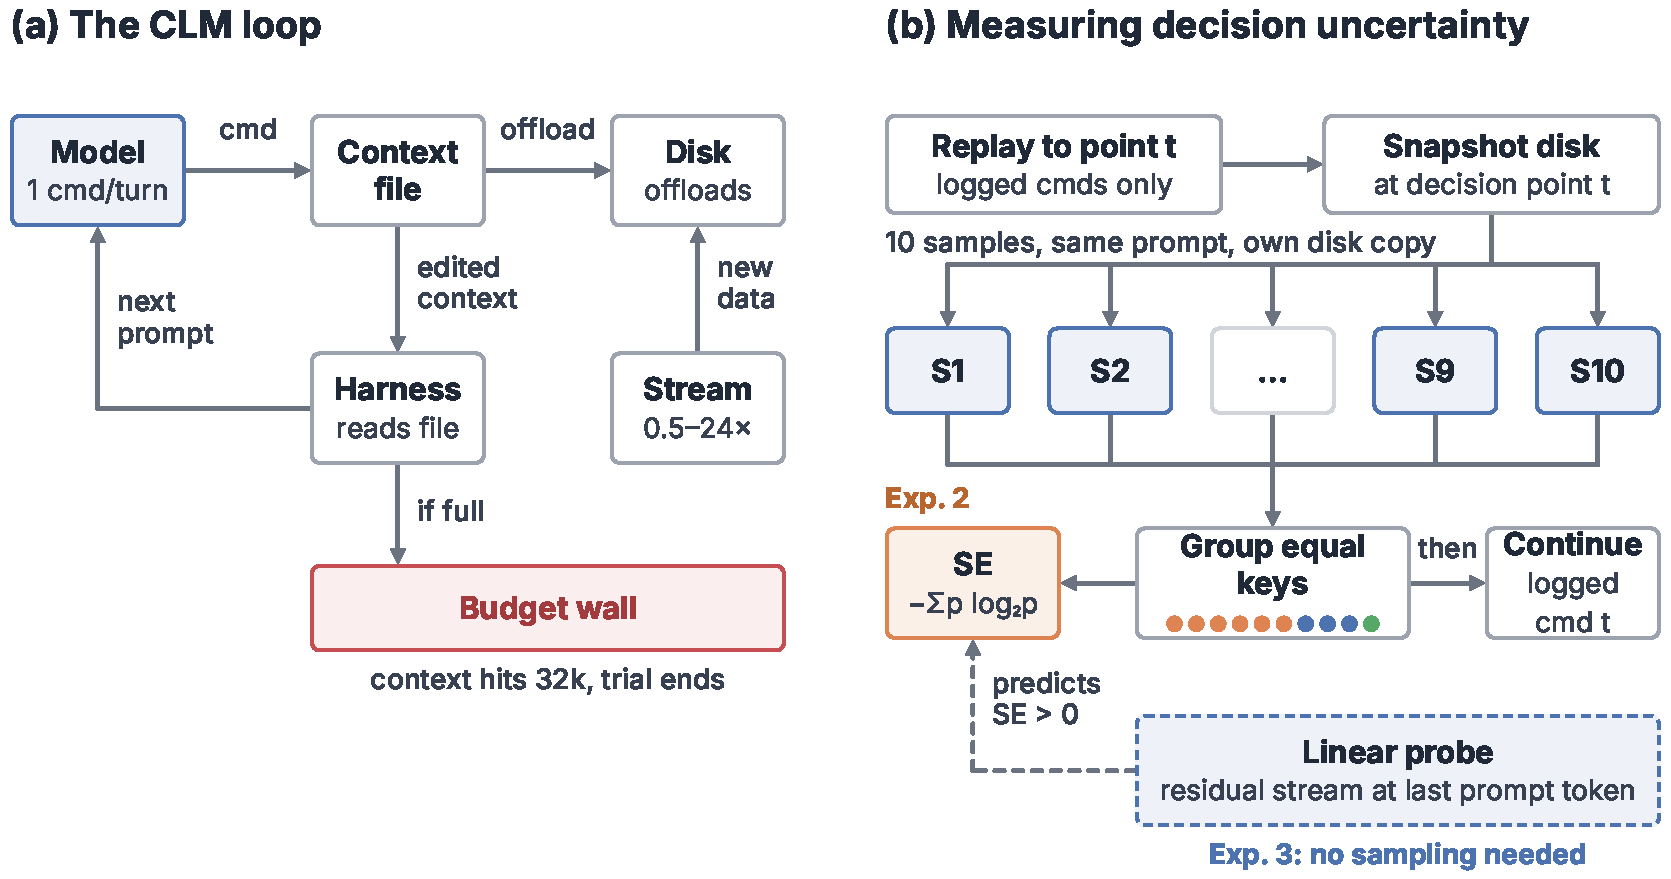
\includegraphics[width=\linewidth]{figs/fig1.pdf}
  \caption{\textbf{(a)} In a CLM, the model edits a file that mirrors its own context.
  Each turn it issues one command that can keep, edit, offload, or delete earlier blocks; the harness reads the edited file back as the next prompt.
  When the context reaches the 32k budget, the trial ends.
  \textbf{(b)} Our measurement.
  A logged trial is replayed without the model up to decision point $t$, where the disk is snapshotted.
  Ten replies sampled from the identical prompt each run on their own copy of the snapshot and receive an outcome key describing their effect on the context.
  Samples with equal keys form one cluster, and semantic entropy is computed over clusters (Experiment~2).
  The replay then continues with the logged command, so the samples never change the trial's path.
  A linear probe reads the same quantity from activations before generation (Experiment~3).}
  \label{fig:schematic}
\end{figure}

\textbf{The CLM harness.} We use the CLM harness and ContextBench of \citet{shao2026clm} (Figure~\ref{fig:schematic}a).
Before each turn the harness writes the editable part of the transcript to a mirror file in which every message is a block headed \texttt{[[CTX\_TURN n role=\ldots]]}.
The model issues exactly one bash command, which runs in a sandbox with persistent shell state.
The harness then reads the mirror back; if the model edited it, the edited text becomes the new message list, unless the edit would grow the context beyond 30{,}720 of 32{,}768 tokens.
The prompt-level instruction \texttt{skill=clm} adds a concrete recipe: write each incoming data batch to a file under \texttt{/tmp/ctx\_offload/} and remove it from the mirror.
The condition \texttt{skill=none} gives only the harness protocol.

\textbf{Tasks and pressure.} We use two ContextBench task families.
In \emph{KV store}, the agent receives a stream of \texttt{SET} batches and must later answer \texttt{GET} queries; in \emph{LogTriage}, it receives log batches and must answer questions about them.
We define \emph{pressure} as the total number of tokens streamed in, divided by the 32{,}768-token budget.
Each family has four levels: KV store R260 / R1000 / R4000 / R16000 (0.46$\times$, 1.57$\times$, 6.04$\times$, 23.9$\times$) and LogTriage L320 / L1600 / L6400 / L12800 (0.51$\times$, 2.2$\times$, 7.9$\times$, 15.8$\times$).
Above 1$\times$ the task cannot fit in context, so the agent must offload or delete.
A trial \emph{hits the budget wall} when its context reaches the limit before the stream ends; the trial then stops and unanswered queries score zero.

\textbf{Models and decoding.} We evaluate Qwen3.5-4B, Qwen3.5-9B, and 9B-RL, the RL checkpoint of the 9B released by \citet{shao2026clm} (\texttt{rl-ckpt-livectx\_dapo-iter44}), which was trained on search tasks rather than ContextBench.
All models are served by vLLM in BF16 with temperature 0.7, top-$p$ 0.95, thinking enabled, and at most 8{,}192 output tokens per turn.
Every LM request and response is logged in full.

%=====================================================================
\section{Experiment 1: Eliciting the failure under context pressure}
\label{sec:exp1}
%=====================================================================

The first experiment establishes that a reimplemented CLM agent fails as pressure rises, and identifies the kind of failure.
We ran 8 seeds per model, family, and level with \texttt{skill=clm} (192 trials), and 4 seeds per cell with \texttt{skill=none} (96 trials).
Success is reward $\geq 0.95$.
We test for a decreasing trend in success with the Cochran--Armitage test on $\log_2$ pressure, and compare slopes between models with a logistic regression \texttt{success $\sim$ model $\times$ $\log_2$(pressure) + family}.

\begin{figure}[!ht]
  \centering
  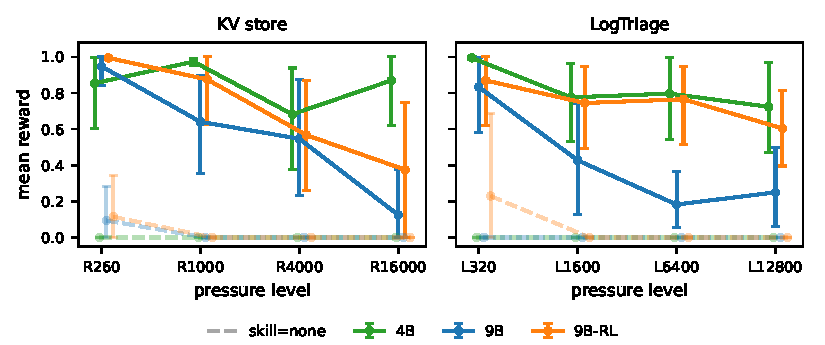
\includegraphics[width=\linewidth]{figs/exp1-reward.pdf}
  \caption{Experiment~1.
  Mean reward against pressure level for the three models with \texttt{skill=clm} (solid, 8 seeds per cell) and \texttt{skill=none} (dashed, 4 seeds per cell).
  Levels 1--4 are R260--R16000 (KV store) and L320--L12800 (LogTriage).
  Error bars: 95\% bootstrap CI of the mean over trials (2{,}000 resamples).}
  \label{fig:exp1}
\end{figure}

\textbf{The 9B degrades with pressure and the 4B does not.} Figure~\ref{fig:exp1} shows that the 9B's mean reward falls from 0.95 to 0.12 on KV store and from 0.83 to 0.18--0.25 on LogTriage across the four levels, and both trends are significant (Cochran--Armitage $z=-2.84$, $p=0.002$ and $z=-3.27$, $p<0.001$).
The 4B, in contrast, stays roughly flat on KV store ($z=0.19$) and declines only weakly on LogTriage ($z=-1.54$, $p=0.06$).
The logistic model confirms that the 9B's odds of success fall faster with pressure than the 4B's (interaction $-0.49$, SE 0.22, $p=0.027$).
The larger model is therefore the more fragile one under pressure, which rules out a simple capacity explanation and points to how each model manages its context.

\textbf{The failures come from context management.} Context management fails in two ways.
In the first, the budget wall, the context fills before the stream ends, and the trial stops with queries unanswered.
This mode dominates, particularly on KV store: above the lowest level, the 9B hit the wall in 28 of 48 trials, against 9 of 48 for the 4B.
In the second, the model reaches the end of the stream but has lost information it needed.
Several 9B LogTriage trials that finished scored about 0.5 because their counts were wrong (L1600 seed 48; L6400 seeds 44, 46, and 49; L12800 seed 45).
In an earlier pilot run we traced this pattern to batches that were removed from context without being offloaded; we did not re-check it for these trials.
The second mode explains why the 9B's LogTriage reward at L6400 (0.18) is lower than its wall count alone implies: only four of eight trials hit the wall, but three of the four that finished scored about 0.5 and the fourth wrote its answers as chat text.
Both modes follow from the model's decisions about what to keep and what to save, which is the behaviour Experiments~2 and~3 examine.

\textbf{RL raises the curve but does not flatten it.} The 9B-RL checkpoint hits the wall about half as often as the base 9B (13 of 48 trials above the lowest level) and scores much higher on LogTriage (0.60--0.87 against 0.18--0.43).
Its slope, however, does not differ from the base model's (interaction $0.09$, $p=0.68$): training shifts the level of performance without removing its dependence on pressure.
This pair of models, with the same architecture and different reliability, is the comparison we carry into Experiment~2.

\textbf{Without the recipe, no model manages its context.} With \texttt{skill=none}, all 96 trials hit the budget wall and 93 score zero.
The models made only 12 context edits in 96 trials, against roughly one per batch with \texttt{skill=clm}.
Context management in these models therefore depends on the instruction, and the variation we study below concerns how well the model follows and adapts a recipe it has been given.
Four zero-reward trials across all conditions were answer-format errors rather than context failures (listed in Appendix~\ref{app:tables}).

%=====================================================================
\section{Measuring uncertainty over context decisions}
\label{sec:method}
%=====================================================================

Token-level confidence is a poor measure of decision uncertainty in this setting, because two commands with different text can have the same effect on the context, and two similar commands can have different effects.
We therefore measure uncertainty over \emph{effects}, which requires executing each sampled command in the state the model saw (Figure~\ref{fig:schematic}b).
Experiments~2 and~3 use 42 logged \texttt{skill=clm} trials per model for the 9B and the 9B-RL, a subset of Experiment~1 covering all eight family--level cells (4--6 seeds per cell).

\textbf{Two kinds of state and byte-exact replay.} The state at turn $t$ has two parts.
The \emph{prompt} determines what the model generates and is logged exactly.
The \emph{disk} (offload files and shell state) determines what a command does, and is not logged because the sandbox is deleted after each trial.
Since only the harness and the model's logged commands write to disk, re-running the logged commands in order in a fresh sandbox with the same root filesystem rebuilds the disk.
After each command we compare the replayed tool output with the logged output; at the first mismatch, the trial is truncated, because later disk states no longer match what the model saw.

\textbf{Decision points and sampling.} A decision point is a logged turn whose command ran.
Per trial we select every turn at which the harness applied a context edit, plus five randomly chosen non-edit turns from each quartile of context fill, up to 40 points; this yields 1{,}409 points for the 9B and 1{,}435 for the 9B-RL.
At each point we resend the logged request unchanged except for $n=10$ samples and a per-point seed, and verify that the server reports the same number of prompt tokens as in the logged call.

\textbf{Execution and labelling.} We replay the trial again, pause before each point's logged command, and snapshot the disk.
Each of the ten sampled commands then runs on its own copy of the snapshot.
A sample receives an \emph{outcome key}.
If the sample did not run normally, the key is a status: \texttt{invalid} (non-zero exit and no context change), \texttt{no\_tool\_call}, \texttt{context\_status}, or \texttt{error}.
Otherwise the key assigns each context block one label: \texttt{stay} (unchanged), \texttt{edit} (partly kept), \texttt{offload} (removed and found in a file the command wrote), or \texttt{delete} (removed and not saved), together with a flag for whether the command destroyed content in a pre-existing file.
Two samples belong to the same semantic cluster if and only if their keys are equal.

\textbf{Semantic entropy.} If cluster $c$ holds a share $p_c$ of the ten samples, the semantic entropy at the point is
\begin{equation}
  \SE = -\sum_c p_c \log_2 p_c ,
\end{equation}
which ranges from 0 bits (all samples agree) to $\log_2 10 \approx 3.32$ bits (all differ).
This is the discrete estimator of \citet{farquhar2024detecting}; it needs cluster frequencies only and measures total uncertainty, without separating aleatoric from epistemic components.
A trial is summarised by its mean SE over points.
Because status outcomes are clusters too, SE combines uncertainty about \emph{which context decision} to make with uncertainty about \emph{whether the command works}.
We therefore also compute \emph{decision-only SE}, the entropy over samples with a normal outcome (points with fewer than two such samples are dropped), and \emph{status-only SE}, the entropy of the status variable with all normal outcomes merged.

\textbf{Validation.} Table~\ref{tab:validation} (Appendix~\ref{app:repro}) lists the checks, all specified before any result was computed.
Replay was byte-identical in 81 of 84 trials.
The three divergences arose from directory metadata (\texttt{ls -la} sizes and timestamps) or an uninspected late turn, and the affected trials were truncated at the divergence.
The labeller, applied to each logged command, reproduced the next logged prompt at every one of 2{,}818 points, which confirms that the outcome keys describe what the harness actually did.
A manual reading of ten labelled 9B points found all ten correct.



%=====================================================================
\section{Experiment 2: Decision uncertainty predicts failure}
\label{sec:exp2}
%=====================================================================

The unit of analysis is the trial.
The test fixed before analysis is the partial Spearman correlation between trial mean SE and reward, controlling for family $\times$ level by rank-residualising both variables on level indicators, with a 95\% CI from 2{,}000 bootstrap resamples over trials.
A secondary OLS regression is \texttt{reward $\sim$ mean SE + C(family:level)}.
One 9B-RL trial that scored zero from an answer-format error, without hitting the wall, is excluded ($n=41$).

\begin{figure}[!ht]
  \centering
  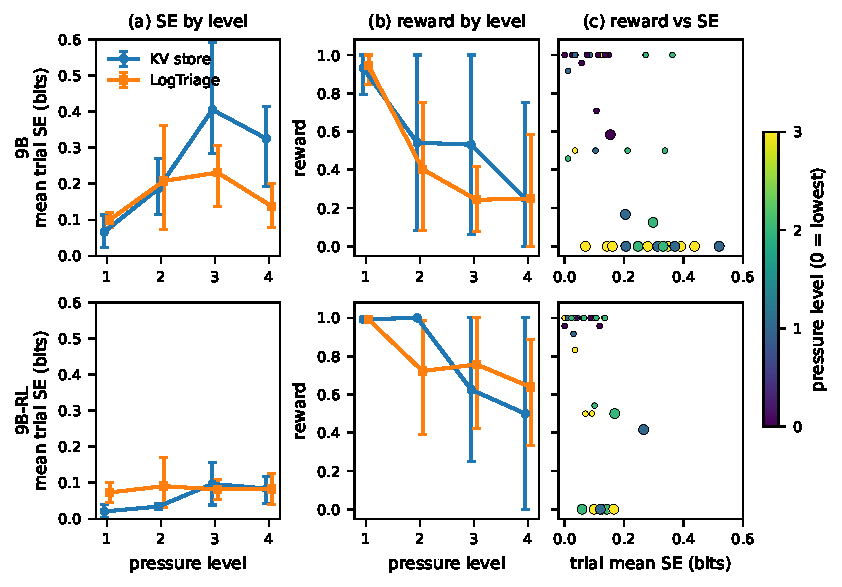
\includegraphics[width=0.75\linewidth]{figs/exp2-se.pdf}
  \caption{Experiment~2.
  Mean trial SE (top) and mean reward (bottom) per pressure level for the 9B and the 9B-RL, shown separately for KV store (left) and LogTriage (right); the two families' levels are not matched in pressure.
  Error bars: 95\% bootstrap CI of the mean over trials (2{,}000 resamples; 4--6 trials per cell).}
  \label{fig:exp2}
\end{figure}

\textbf{Most decisions are certain, and uncertainty concentrates where pressure is high.} At most points all ten samples take the same action: the share of points with SE $=0$ ranges from 50\% to 91\% per cell for the 9B and from 84\% to 96\% for the 9B-RL.
The offload recipe of \texttt{skill=clm} dominates the model's behaviour, so the informative variation lies in a minority of points.
For the 9B, mean SE rises from 0.07--0.10 bits at the lowest level to 0.23--0.41 bits at level 3, then falls at level 4 (Figure~\ref{fig:exp2}, top).
A plausible explanation for the final drop, which we have not tested, is that level-4 trials hit the wall early and therefore contribute fewer edit decisions.

\textbf{At fixed pressure, more uncertain trials score lower.} Table~\ref{tab:h1} reports the main test.
In the 9B, the partial correlation between mean SE and reward is $\rho=-0.587$ (95\% CI $[-0.775,-0.282]$), and adding SE to the pressure indicators raises $R^2$ from 0.40 to 0.66.
In practical terms, at a fixed level, a trial whose decisions carry 0.1 bits more mean SE scores about 0.20 lower.
Pressure sets the average difficulty, and the model's inconsistency about its own context decisions separates the trials that cope from those that do not.

\begin{table}[!ht]
  \centering
  \small
  \caption{Experiment~2: association between trial mean SE and reward at fixed pressure.
  Partial Spearman $\rho$ with 95\% bootstrap CI over trials; OLS coefficients with $p$-values.}
  \label{tab:h1}
  \begin{tabular}{@{}lll@{}}
    \toprule
    Measure & 9B ($n=42$) & 9B-RL ($n=41$) \\
    \midrule
    Mean SE (test fixed in advance) & $\mathbf{-0.587}$ $[-0.775,-0.282]$ & $\mathbf{-0.477}$ $[-0.736,-0.094]$ \\
    Max SE & $-0.42$ $[-0.72,-0.05]$ & $-0.355$ $[-0.723,+0.065]$ \\
    Decision-only SE & $-0.496$ $[-0.731,-0.120]$ & $-0.446$ $[-0.698,-0.063]$ \\
    Status-only SE & $-0.472$ $[-0.675,-0.218]$ & $-0.287$ $[-0.618,+0.116]$ \\
    \midrule
    OLS SE coefficient ($p$); $\Delta R^2$ over level & $-2.02$ ($<0.001$); $+0.26$ & $-3.16$ ($0.003$); $+0.19$ \\
    \quad + context fill and number of points & $-1.65$ ($0.0003$) & $-3.02$ ($0.006$) \\
    Joint OLS: decision / status coefficient ($p$) & $-1.50$ ($0.010$) / $-2.85$ ($0.004$) & $-5.59$ ($0.004$) / $+0.54$ ($0.82$) \\
    \bottomrule
  \end{tabular}
\end{table}

\textbf{The association is not a proxy for context length.} If SE merely tracked how full the context was, it would add nothing once fill is controlled.
Adding mean context fill and the number of decision points to the regression leaves the SE coefficient significant in both models ($-1.65$ and $-3.02$).
At the level of individual points, SE correlates only weakly with fill (Spearman 0.20 for the 9B, 0.03 for the 9B-RL), and non-zero SE occurs at every fill level.
The correlation also holds within each family for the 9B (KV store $\rho=-0.78$, LogTriage $\rho=-0.51$) and separately on edit turns ($-0.45$) and non-edit turns ($-0.42$).

\textbf{The association is not explained by failed commands.} Because SE counts failed commands and malformed tool calls as clusters, a high-SE trial might simply be one in which the model writes broken commands.
Restricting SE to samples whose command ran normally answers this objection: decision-only SE still predicts reward in both models ($\rho=-0.496$ and $-0.446$, both CIs excluding zero), and it correlates with total SE at 0.93 and 0.91 at the trial level.
Uncertainty about the context decision itself is therefore sufficient for the effect.
The two components behave differently across models.
In the 9B, uncertainty about command success is a second, partly independent predictor (joint OLS $p=0.004$); in the 9B-RL it adds nothing ($p=0.82$), which suggests that RL training removed most command failures while leaving some uncertainty about what to keep.

\textbf{High-SE points are real dilemmas.} The five highest-SE points in the development trials (1.29--1.57 bits) each mixed three courses of action: offloading the incoming batch as the recipe prescribes, answering a pending query first, or removing a different set of earlier turns (for example, deleting six old blocks rather than shortening three).
The choice among them decides which information survives.

\textbf{RL reduces uncertainty, and the remainder still matters.} Across all eight cells, the 9B-RL's mean SE is 60--80\% lower than the 9B's, its reward is higher (at level 4: 0.50 against 0.25 on KV store, 0.64 against 0.25 on LogTriage), and fewer of its trials hit the wall (8 against 18).
The rise of SE with pressure seen in the 9B disappears.
Despite the narrower range, the residual uncertainty predicts failure with a larger per-bit coefficient ($-3.16$ against $-2.02$).
A comparison of two checkpoints cannot establish that lower uncertainty causes the higher reward, but the pattern is consistent with uncertainty being one route to failure that RL training partially closes.

\textbf{Limits of the evidence.} SE computed only from the first half of each trial predicts reward weakly in the 9B ($\rho=-0.24$; OLS $p=0.028$ when controlling for first-half fill, $p=0.18$ with whole-trial fill) and not at all in the 9B-RL ($\rho=-0.10$), so we cannot claim that uncertainty reliably precedes failure.
The planned step-level test was also uninformative, because our harmful-edit proxy marked 92--93\% of edit turns as harmful.

%=====================================================================
\section{Experiment 3: Decision uncertainty is linearly decodable}
\label{sec:exp3}
%=====================================================================

Measuring SE requires ten samples and ten executions per decision.
Experiment~3 asks whether the same information is present in the activations before generation, as \citet{kossen2024sep} found for hallucination.

\textbf{Probe setup.} For every decision point we run a forward pass on the logged prompt and logged reply and record the residual stream at all 32 decoder layers, at two positions: the last prompt token (TBG, before generation) and the last reply token (SLT).
Prompt token counts match the vLLM log at every point.
The binary target is SE $>0$ (logistic regression, $C=0.05$, scored by AUROC); the threshold that minimises within-group squared error is 0 bits, and 30\% of 9B points and 12\% of 9B-RL points are positive.
The continuous target is SE itself (ridge regression, $\alpha=1000$, scored by Spearman correlation).
Evaluation uses 5-fold cross-validation grouped by trial, so no trial appears in both training and test folds, and the layer is chosen within the training folds.
As controls, we train the same probe on context fill and turn index alone, and on shuffled labels.

\begin{table}[!ht]
  \centering
  \small
  \caption{Experiment~3: linear probes on the residual stream, 5-fold cross-validation grouped by trial.
  TBG = last prompt token; SLT = last reply token.
  The control probe uses context fill and turn index only.
  Decision-only rows use a fixed layer (20 for the 9B, 28 for the 9B-RL).}
  \label{tab:probe}
  \begin{tabular}{@{}llcccc@{}}
    \toprule
    & & \multicolumn{2}{c}{9B} & \multicolumn{2}{c}{9B-RL} \\
    \cmidrule(lr){3-4}\cmidrule(lr){5-6}
    Target & Position & Probe & Control & Probe & Control \\
    \midrule
    SE $>0$ (AUROC) & TBG & \textbf{0.741} & 0.578 & \textbf{0.818} & 0.493 \\
    SE $>0$ (AUROC) & SLT & 0.648 & -- & 0.729 & -- \\
    SE (Spearman) & TBG & 0.466 & 0.159 & 0.383 & 0.004 \\
    SE residualised on fill (Spearman) & TBG & 0.371 & -- & 0.238 & -- \\
    Decision-only SE $>0$ (AUROC) & TBG & \textbf{0.766} & 0.520 & \textbf{0.809} & 0.487 \\
    Decision-only SE (Spearman) & TBG & 0.433 & 0.048 & 0.347 & $-0.006$ \\
    Status-only SE $>0$ (AUROC) & TBG & 0.741 & 0.675 & 0.833 & 0.545 \\
    Shuffled labels, SE $>0$ (AUROC) & TBG & 0.483 & -- & 0.522 & -- \\
    \bottomrule
  \end{tabular}
\end{table}

\textbf{The model's hidden state predicts whether its next decision will be uncertain.} Table~\ref{tab:probe} shows that a linear probe at the last prompt token predicts SE $>0$ with AUROC 0.741 in the 9B (best layers 18--20) and 0.818 in the 9B-RL (layer 28).
Shuffled labels give chance performance (0.48 and 0.52), so the result does not come from the probe fitting noise.

\textbf{The signal goes beyond context length.} The control probe on fill and turn index reaches 0.578 in the 9B and 0.493 in the 9B-RL, well below the activation probe, and after SE is residualised on fill the probe still recovers it (Spearman 0.371 in the 9B).
In the 9B-RL, context length carries no information about SE at all, yet the activation probe performs best.
The decoded quantity is therefore not the length confound described by \citet{du2025context}.

\textbf{The uncertainty is present before generation.} In both models the probe at the last prompt token outperforms the probe at the last reply token (0.741 against 0.648; 0.818 against 0.729), the same ordering \citet{kossen2024sep} report for hallucination.
The representation of uncertainty is thus formed while the model reads its context, before it reasons or writes a command.

\textbf{Decision uncertainty specifically is decodable.} With decision-only SE as the target, the probe reaches AUROC 0.766 (9B) and 0.809 (9B-RL), while the control falls to chance (0.520 and 0.487).
Uncertainty about command success is also decodable, but in the 9B it is partly predictable from context length alone (control 0.675).
The component of uncertainty that concerns what to keep in context is the one least explained by length and best explained by the model's internal state.

%=====================================================================
\section{Discussion}
\label{sec:discussion}
%=====================================================================

The three experiments form one chain of evidence: CLM agents fail under pressure because of how they manage context, either by filling it or by dropping information they later need (Experiment~1); at the same pressure, trials in which the model is less consistent about its context decisions score lower (Experiment~2); and this uncertainty is linearly encoded before the model acts and is not reducible to context length (Experiment~3).
A model that edits its context decides which evidence its future self will see, and our results show that it carries information about when those decisions are unreliable, even though its output does not report it.


\textbf{Implications.} If uncertainty about context decisions is both predictive of failure and cheaply readable, it can be used to make context management safer.
We outline four directions that our results motivate but do not test.
(i) \emph{Uncertainty-gated edits}: when the probe or a sampled SE estimate exceeds a threshold, the harness can convert a deletion into an offload, so that an uncertain decision remains reversible, or defer the edit until more information arrives.
(ii) \emph{Explicit uncertainty annotations}: the model or the harness can attach an uncertainty score to each block in the context file, so that later turns know which earlier decisions were tentative.
(iii) \emph{Deployer-set thresholds}: the threshold in (i) is one interpretable parameter that trades context budget against the risk of irreversible loss.
(iv) \emph{Training and monitoring}: because RL reduced decision uncertainty alongside failure, SE or its probe could serve as an auxiliary training signal, and a probe could flag agents whose memory management is becoming unreliable during deployment.

\textbf{Limitations.} Four limitations bound these conclusions; Appendix~\ref{app:limitations} gives the full list.
First, the evidence is correlational.
A preliminary ablation of the 9B's uncertainty direction \citep{arditi2024refusal} made context decisions slightly more consistent when the direction was halved, but the direction is partly aligned with context length and the dose response is not monotonic, so we treat it as exploratory (Appendix~\ref{app:h3}).
Second, SE measures total predictive uncertainty: it does not separate epistemic uncertainty (what the model does not know) from aleatoric uncertainty (several equally valid decisions), so some high-SE points may reflect interchangeable choices rather than ignorance.
Third, the offload recipe makes 50--96\% of decisions per cell certain, each SE value rests on ten samples, and each model contributes only 42 trials, which narrows the range of SE and widens the confidence intervals.
Fourth, the analysis covers one model family, one instruction condition, and two task families, and we have no step-level ground truth for which individual decisions cause failure.

%=====================================================================
\section{Conclusion}
%=====================================================================

On ContextBench, the semantic entropy of a CLM's context-management decisions, measured by executing resampled commands and clustering them by their effect on the context, predicts task failure beyond pressure level ($\rho=-0.587$ for Qwen3.5-9B and $-0.477$ for its RL checkpoint), and a linear probe recovers it from the residual stream before generation (AUROC 0.741 and 0.818).
Testing whether acting on this signal (Section~\ref{sec:discussion}) prevents failures, and establishing the causal role of the uncertainty direction, are the next steps.


\begin{ack}
  This work is supported and funded by the Pathfinder Fellowship, a program run by Kairos.
  The author thanks the Nanyang AI Safety group at Nanyang Technological University (NTU) for their feedback and support.
\end{ack}

\clearpage
\bibliographystyle{plainnat}
\bibliography{refs}

\clearpage
\appendix

%=====================================================================
\section{Limitations and dual-use / ethical considerations}
\label{app:limitations}
%=====================================================================

\textbf{Limitations (full list).}
\begin{enumerate}
    \item \emph{Correlational evidence.} Experiments~2 and~3 establish association and decodability, not causation.
    The intervention in Appendix~\ref{app:h3} is preliminary and confounded with context length.
    \item \emph{Recipe floor.} Between 50\% and 96\% of points per cell have SE $=0$, because the offload recipe dominates.
    SE therefore has a narrow range, and the probe labels are imbalanced.
    \item \emph{Noisy point estimates.} Each SE value is computed from ten samples, which bounds the attainable probe accuracy and makes individual point values unreliable.
    \item \emph{Sample size.} The trial-level analysis has 42 trials per model (41 for the 9B-RL), with 4--6 trials per cell; confidence intervals are correspondingly wide.
    \item \emph{No step-level ground truth.} Our harmful-edit proxy was uninformative, so we do not identify which individual decisions cause failure.
    \item \emph{Scope.} Experiments~2 and~3 cover one model family (Qwen3.5-9B and its RL checkpoint), one instruction condition (\texttt{skill=clm}), and two task families.
    The 9B-RL checkpoint was trained on search tasks, so its ContextBench behaviour is out of distribution.
    \item \emph{Total, not epistemic, uncertainty.} Discrete SE estimates the model's total predictive uncertainty.
    It does not separate epistemic uncertainty, which arises from what the model does not know about the task or its context, from aleatoric uncertainty, which arises when several decisions are equally valid (for example, two acceptable ways to shorten the context).
    Some high-SE points may therefore reflect interchangeable choices rather than ignorance, and our results should be read as statements about total uncertainty; we make no claim that the uncertainty we measure is epistemic.
    The headline SE also mixes decision and command-success uncertainty; the decision-only analysis separates these two, but not the epistemic and aleatoric components.
    \item \emph{Probe directions.} At layer 20 the logistic probe direction and the difference-of-means direction are nearly orthogonal (cosine 0.09), so which direction is causally relevant remains open.
\end{enumerate}

\textbf{Dual-use and ethical considerations.} The work characterises when a model is uncertain about its own memory management and locates a representation of that uncertainty.
Two misuse routes follow from the same findings.
First, an intervention on the uncertainty direction could make a model act with unwarranted confidence when it deletes information, which would remove the signal that our proposed safeguards rely on.
Second, knowledge of what a probe reads could be used to train or fine-tune a model so that its uncertainty becomes invisible to such a monitor while its behaviour is unchanged.
Both risks argue for treating uncertainty monitors as one layer of oversight among several, and for preferring reversible actions (offload over delete) by default.
The experiments use synthetic benchmark data with no personal information, and the models and benchmark are publicly released.
All compute ran on rented GPUs within a fixed budget.

%=====================================================================
\section{Per-cell results}
\label{app:tables}
%=====================================================================

\begin{table}[!ht]
  \centering
  \small
  \caption{Experiment~1, \texttt{skill=clm}: mean reward, successes (reward $\geq 0.95$), and budget-wall trials, 8 seeds per cell.}
  \begin{tabular}{@{}llccc|ccc|ccc@{}}
    \toprule
    & & \multicolumn{3}{c}{4B} & \multicolumn{3}{c}{9B} & \multicolumn{3}{c}{9B-RL} \\
    Family & Level & Rew. & Succ. & Wall & Rew. & Succ. & Wall & Rew. & Succ. & Wall \\
    \midrule
    KV & R260 (0.46$\times$) & 0.85 & 6 & 0 & 0.95 & 7 & 1 & 0.99 & 8 & 0 \\
    KV & R1000 (1.57$\times$) & 0.97 & 7 & 0 & 0.64 & 4 & 4 & 0.88 & 7 & 0 \\
    KV & R4000 (6.04$\times$) & 0.68 & 5 & 3 & 0.55 & 4 & 4 & 0.57 & 4 & 4 \\
    KV & R16000 (23.9$\times$) & 0.87 & 7 & 1 & 0.12 & 1 & 7 & 0.38 & 3 & 5 \\
    LogTriage & L320 (0.51$\times$) & 0.99 & 8 & 0 & 0.83 & 6 & 1 & 0.87 & 7 & 0 \\
    LogTriage & L1600 (2.2$\times$) & 0.78 & 5 & 1 & 0.43 & 2 & 4 & 0.74 & 3 & 2 \\
    LogTriage & L6400 (7.9$\times$) & 0.80 & 6 & 2 & 0.18 & 0 & 4 & 0.77 & 5 & 1 \\
    LogTriage & L12800 (15.8$\times$) & 0.72 & 5 & 2 & 0.25 & 1 & 5 & 0.60 & 2 & 1 \\
    \bottomrule
  \end{tabular}
\end{table}

Four zero-reward trials were not context-management failures: the 4B at KV R260 wrote every answer to \texttt{/dev/null}; the 9B-RL at KV R1000 stripped a checksum suffix from every value; the 9B-RL at LogTriage L320 emitted a malformed answer tag; and one 9B LogTriage L6400 trial wrote answers as chat text.

\begin{table}[!ht]
  \centering
  \small
  \caption{Experiments~2--3 subset: per-cell reward, budget-wall trials, mean SE (bits), and share of points with SE $=0$.}
  \begin{tabular}{@{}lc|cccc|cccc@{}}
    \toprule
    & & \multicolumn{4}{c}{9B} & \multicolumn{4}{c}{9B-RL} \\
    Cell & $n$ & Rew. & Wall & SE & SE$=0$ & Rew. & Wall & SE & SE$=0$ \\
    \midrule
    KV R260 & 6 & 0.93 & 1 & 0.07 & 0.91 & 0.99 & 0 & 0.02 & 0.96 \\
    KV R1000 & 4 & 0.54 & 2 & 0.19 & 0.70 & 1.00 & 0 & 0.03 & 0.95 \\
    KV R4000 & 4 & 0.53 & 2 & 0.41 & 0.50 & 0.63 & 2 & 0.10 & 0.84 \\
    KV R16000 & 4 & 0.25 & 3 & 0.33 & 0.55 & 0.50 & 2 & 0.08 & 0.86 \\
    LogTriage L320 & 6 & 0.94 & 0 & 0.10 & 0.82 & 0.99 & 0 & 0.07 & 0.89 \\
    LogTriage L1600 & 6 & 0.40 & 3 & 0.21 & 0.71 & 0.72 & 2 & 0.09 & 0.87 \\
    LogTriage L6400 & 6 & 0.24 & 3 & 0.23 & 0.67 & 0.76 & 1 & 0.08 & 0.86 \\
    LogTriage L12800 & 6 & 0.25 & 4 & 0.14 & 0.78 & 0.64 & 1 & 0.08 & 0.89 \\
    \bottomrule
  \end{tabular}
\end{table}

%=====================================================================
\section{Preliminary intervention on the uncertainty direction}
\label{app:h3}
%=====================================================================

We took the difference of mean activations at the last prompt token between points with SE $>0$ and SE $=0$ in the 9B at layer 20, normalised it to a unit vector $d$, and scaled it in every matrix that writes to the residual stream (the embedding and each layer's attention and MLP output projections; 65 matrices) via $W \leftarrow (I + (\lambda-1)dd^\top)W$.
Here $\lambda=0$ removes the direction and $\lambda=0.5$ halves it.
The edited model was resampled at the same decision points with the same seeds on a subset of 16 trials (two per cell, 547 points), and compared point by point with the unedited baseline.

\begin{table}[!ht]
  \centering
  \small
  \caption{Change in decision-only SE relative to the unedited 9B (Wilcoxon signed-rank test over points; per-trial mean change with 95\% bootstrap CI).}
  \begin{tabular}{@{}lccc@{}}
    \toprule
    Condition & Format fail. & $\Delta$ dec.-only SE ($p$) & Per trial [95\% CI] \\
    \midrule
    Random direction, $\lambda=0$ (42 trials) & 0.2\% & $-0.007$ (0.56) & $-0.006$ $[-0.015,+0.003]$ \\
    SE direction, $\lambda=0.5$ & 0.1\% & $-0.062$ (0.0001) & $-0.053$ $[-0.090,-0.021]$ \\
    SE direction, $\lambda=0$ & $\approx$48\% & $+0.18$ ($10^{-10}$) & $+0.17$ $[+0.10,+0.26]$ \\
    \bottomrule
  \end{tabular}
\end{table}

Halving the direction leaves tool use intact and makes context decisions slightly more consistent; the effect comes from LogTriage, while KV store moves slightly in the opposite direction.
Removing the direction entirely breaks the tool-call format in about half of the samples, and when we resample until ten well-formed calls are obtained (9 trials), decision-only SE still rises (0.145 to 0.423 bits).
We do not treat these results as evidence of causality, for three reasons.
The direction is partly a context-length direction (cosine 0.45 with the fill direction; 31\% of its squared norm lies in the span of fill, task family, and turn type) and was built from SE that includes failed commands.
The random control removes far less of the residual stream than the SE direction (projection spread 0.28 against 7.06).
And the dose response is not monotonic.
A cleaner test would build the direction from decision-only SE on activations residualised for fill, task, and turn type, compare it with a matched context-length direction, and measure task reward under amplification.

%=====================================================================
\section{Reproducibility}
\label{app:repro}
%=====================================================================

\textbf{Settings.} Context budget 32{,}768 tokens with a 2{,}048-token reserve; no step cap; vLLM 0.33.0, BF16, prefix caching; sandbox root filesystem \texttt{python:3.12-slim} (digest \texttt{sha256:05a994d2\ldots}).
The 9B-RL checkpoint is \texttt{context-language-model/rl-ckpt-livectx\_dapo-iter44} at revision \texttt{ffc4aab2}.
Probes: logistic regression with $C=0.05$ and ridge regression with $\alpha=1000$ on standardised activations; layer selected by inner cross-validation.

\begin{table}[!ht]
  \centering
  \small
  \caption{Validation of the measurement pipeline.}
  \label{tab:validation}
  \begin{tabular}{@{}lll@{}}
    \toprule
    Check & 9B & 9B-RL \\
    \midrule
    Replay fidelity (tool output identical to log) & 40 / 42 trials & 41 / 42 trials \\
    Labeller reproduces next logged prompt & 1{,}397 / 1{,}397 points & 1{,}421 / 1{,}421 points \\
    Resampled prompt tokens equal logged & 1{,}409 / 1{,}409 points & 1{,}435 / 1{,}435 points \\
    Execution errors in samples & 0 / 14{,}090 & 0 / 14{,}350 \\
    Manual check of labels & 10 / 10 correct & -- \\
    \bottomrule
  \end{tabular}
\end{table}

\textbf{Code and provenance.} The CLM harness and ContextBench are third-party code from \citet{shao2026clm}.
The reimplementation, logging proxy, replay and labelling pipeline, analysis, and probes were written during the research sprint and are available at \url{https://github.com/ebenl08/clm-epistemics/}.

%=====================================================================
\section{LLM usage statement}
\label{app:llm}
%=====================================================================

This project made extensive use of an agentic AI coding tool, Claude Code (Anthropic), throughout the research sprint.
The tool wrote and ran most of the experiment code under the author's direction: the reimplementation of the CLM harness setup, the logging proxy, the replay, sampling, and labelling pipeline, the statistical analysis, the probes, and the figures.
It also launched and monitored the GPU jobs, summarised literature, and drafted and edited the text of this paper, including the LaTeX source and the schematic in Figure~\ref{fig:schematic}.
The author designed the research questions and experiments, decided which analyses to run and report, reviewed the code and outputs, and checked the reported numbers against the analysis outputs and the references against their sources.
The author takes full responsibility for the content of the paper.

\end{document}
